%%
%% This is file `sample-sigconf.tex',
%% generated with the docstrip utility.
%%
%% The original source files were:
%%
%% samples.dtx  (with options: `sigconf')
%% 
%% IMPORTANT NOTICE:
%% 
%% For the copyright see the source file.
%% 
%% Any modified versions of this file must be renamed
%% with new filenames distinct from sample-sigconf.tex.
%% 
%% For distribution of the original source see the terms
%% for copying and modification in the file samples.dtx.
%% 
%% This generated file may be distributed as long as the
%% original source files, as listed above, are part of the
%% same distribution. (The sources need not necessarily be
%% in the same archive or directory.)
%%
%%
%% Commands for TeXCount
%TC:macro \cite [option:text,text]
%TC:macro \citep [option:text,text]
%TC:macro \citet [option:text,text]
%TC:envir table 0 1
%TC:envir table* 0 1
%TC:envir tabular [ignore] word
%TC:envir displaymath 0 word
%TC:envir math 0 word
%TC:envir comment 0 0 
%%
%%
%% The first command in your LaTeX source must be the \documentclass
%% command.
%%
%% For submission and review of your manuscript please change the
%% command to \documentclass[manuscript, screen, review]{acmart}.
%%
%% When submitting camera ready or to TAPS, please change the command
%% to \documentclass[sigconf]{acmart} or whichever template is required
%% for your publication.
%%
%%

\documentclass[sigconf]{acmart}
\usepackage[linesnumbered,ruled,vlined]{algorithm2e}
\usepackage{subfigure}
\usepackage{graphicx}
%%
%% \BibTeX command to typeset BibTeX logo in the docs
\AtBeginDocument{%
  \providecommand\BibTeX{{%
    Bib\TeX}}}

%% Rights management information.  This information is sent to you
%% when you complete the rights form.  These commands have SAMPLE
%% values in them; it is your responsibility as an author to replace
%% the commands and values with those provided to you when you
%% complete the rights form.
\setcopyright{acmlicensed}
\copyrightyear{2018}
\acmYear{2018}
\acmDOI{XXXXXXX.XXXXXXX}

%% These commands are for a PROCEEDINGS abstract or paper.
\acmConference[Conference acronym 'XX]{Make sure to enter the correct
  conference title from your rights confirmation emai}{June 03--05,
  2018}{Woodstock, NY}
%%
%%  Uncomment \acmBooktitle if the title of the proceedings is different
%%  from ``Proceedings of ...''!
%%
%%\acmBooktitle{Woodstock '18: ACM Symposium on Neural Gaze Detection,
%%  June 03--05, 2018, Woodstock, NY}
\acmISBN{978-1-4503-XXXX-X/18/06}


%%
%% Submission ID.
%% Use this when submitting an article to a sponsored event. You'll
%% receive a unique submission ID from the organizers
%% of the event, and this ID should be used as the parameter to this command.
%%\acmSubmissionID{123-A56-BU3}

%%
%% For managing citations, it is recommended to use bibliography
%% files in BibTeX format.
%%
%% You can then either use BibTeX with the ACM-Reference-Format style,
%% or BibLaTeX with the acmnumeric or acmauthoryear sytles, that include
%% support for advanced citation of software artefact from the
%% biblatex-software package, also separately available on CTAN.
%%
%% Look at the sample-*-biblatex.tex files for templates showcasing
%% the biblatex styles.
%%

%%
%% The majority of ACM publications use numbered citations and
%% references.  The command \citestyle{authoryear} switches to the
%% "author year" style.
%%
%% If you are preparing content for an event
%% sponsored by ACM SIGGRAPH, you must use the "author year" style of
%% citations and references.
%% Uncommenting
%% the next command will enable that style.
%%\citestyle{acmauthoryear}


%%
%% end of the preamble, start of the body of the document source.
\begin{document}

%%
%% The "title" command has an optional parameter,
%% allowing the author to define a "short title" to be used in page headers.
\title{Compression Distance for Anomaly Detection}

%%
%% The "author" command and its associated commands are used to define
%% the authors and their affiliations.
%% Of note is the shared affiliation of the first two authors, and the
%% "authornote" and "authornotemark" commands
%% used to denote shared contribution to the research.
\author{Charles Meyers}
\email{cmeyers@cs.umu.se}
\affiliation{%
  \institution{Umeå University}
  \city{Umeå}
  \country{Sweden}
}
\author{Aaron P. MacSween}
\email{publishing@cryptography.dog}
\affiliation{
    \institution{null}
    \city{na}
    \country{undefined}
}
\author{Tommy Löfstedt}
\email{tommy@cs.umu.se}
% \affiliation{%
%   \institution{Umeå University}
%   \city{Umeå}
%   \country{Sweden}
% }
\author{Erik Elmroth}
\email{elmroth@cs.umu.se}
% \affiliation{%
%   \institution{Umeå University}
%   \city{Umeå}
%   \country{Sweden}
% }

% \affiliation{%
%   \institution{Umeå University}
%   \city{Umeå}
%   \country{Sweden}
%   \country{USA}
%   \postcode{43017-6221}
% }

\begin{abstract}
  Machine learning have proven remarkable performance across a wide variety of domains, but nevertheless fail to adversaries during model training or deployment. 
  Recent developments have focused on incredibly complex architectures with long run-times, specific hardware requirements, and models that leak private information to anyone with access to the API. 
  However, the use of compression algorithms in conjunction with clustering algorithms has proven remarkably successful at text classification, excelling in few-show circumstances and across a wide-variety of datasets. This makes it ideal for a private anomaly detection algorithm. In this paper, we show how a client-side approach to anomaly detection is safer by design.
  In addition, we demonstrate the efficacy of this technique in the domain of computer security---using datasets spanning computer processes, Twitter bots, intrusion attacks, denial of service attacks, and log file outlier detection.
  We offer advice for improving the model latency and evaluate NCD in the wider context of kernel metrics to show its broad efficacy.
    
\end{abstract}


\keywords{ML for Security, Security of ML, Adversarial Attacks, Anomaly Detection, DDOS Detection, Bot Detection}



% \received{\date{\today}}
% \received[revised]{12 March 2009}
% \received[accepted]{5 June 2009}

%%
%% This command processes the author and affiliation and title
%% information and builds the first part of the formatted document.
\maketitle

\section{Introduction}

Despite their efficacy across many domains, modern machine learning methods often use very large models that require large numbers of samples to train \cite{desislavov2021compute}. The exchange of this data often creates privacy and security risks \cite{}. For example, several attacks against ML systems have been proposed, targeting the model during training \cite{biggio_poisoning_2013}, prediction \cite{biggio_evasion_2013,deepfool,carlini_towards_2017}, or deployment \cite{distributed_attacks,santos2021universal}. Even when access to a model is limited only to the classification labels, it is possible to subvert the model \cite{hopskipjump}, reverse engineer the decision boundary \cite{deepfool}, determine the model weights \cite{jagielski2020high} or infer the class-membership of new samples \cite{bentley2020quantifying}. This raises profound questions for safety critical systems \cite{meyers} and legal questions about access and control of the underlying data \cite{mitrou2018data,marks2023ai}. One solution to the problem of adversaries is to treat the model as we would treat a session token or any other private data-- by keeping it encrypted locally and providing no access in either direction to the internet. However, this lack of data sharing means that our method must work well when trained on a small number of samples to minimize the run-time costs and maximize the efficacy for individual users.  Luckily, Jiang et al.\cite{jiang2022less} proposed a parameter-free text classification algorithm that exploits the compression algorithm, DEFLATE, to compress and then classify strings that has shown very strong performance against several benchmark datasets. In this study, we explore the underlying theory of kernel methods, offer run-time improvements over the original\cite{jiang2022less} GZIP-KNN classifier, demonstrate the efficacy of our run-time optimized method on a variety of datasets comprised of a variety of data types to provide a plausible model for private and client-side anomaly detection.

\subsection{Motivations}
 We have several motivations for this work. Firstly, Jiang's analysis relies on many thousands of samples and it's unclear how well it performs in the few-shot circumstances. While follow-up research examined topics like image classification \cite{opitz2023gzip}, chemical classification \cite{weinreich2023parameter}, and text classification \cite{nishida2011tweet}, it has not been explored in the context of anomaly detection. Furthermore, if we can minimize the run-time storage and computation requirements, then we can fulfill our goal of deploying this method entirely client-side.

\subsection{Contributions}

In this study, we:

\begin{itemize}
    \item Explore the theory behind the gzip-knn 
    \item Demonstrate how private model deployment is safer by design(Sec.~\ref{threat})
    \item Offer run-time improvements over the GZIP-KNN classifier (Sec.~\ref{improvements})
    \item Provide a live example of the model in javascript as well as a scikit-learn implementation
    \item demonstrate the efficacy of the GZIP-KNN classifier across several anomaly detection datasets
    \item We also demonstrate the efficacy of the run-time optimizations
\end{itemize}

\subsection{Definitions}
\paragraph{Distance}
Distance refers to any norm or pseudo-norm for measuring the proximity of one sample to another. 
% \paragraph{Benign vs Adversarial}
\paragraph{Failure Rate}
We will define the failure rate
\paragraph{Survival Time}

\section{GZIP-KNN}
In this section, we reproduce the GZIP-KNN algorithm proposed by Jiang et al. to inform a run-time analysis of the algorithm and offer insights towards our  improvements that are outlined in Sec~\ref{improvements}. Broadly, this method uses a widely-researched clustering model, $k$-Nearest Neighbors, in conjunction with a  distance metric called \textit{normalized compression distance} (NCD). 


\subsection{GZIP}
    The \texttt{gzip} package is an open-source and widely available software tool for compressing files \cite{gzip} that uses the DEFLATE compression algorithm \cite{deflate}. It uses a sliding window dictionary and Huffman coding \cite{} to compress data into an output buffer by reading the symbols one at a time. Then, it iterates through the data. If the current symbol is in the sliding window dictionary, then it will add it to the output buffer. Otherwise, it finds the longest matching sequence of symbols in the window, encodes them using Huffman coding, and removes the matches symbols from the output buffer, before adding the new key to the sliding window dictionary. The full algorithm can be found in the original paper, here\cite{deflate}.
% \begin{algorithm}
%   \KwData{Input data stream $input\_data$}
%   \KwResult{Compressed data stream $compressed\_data$}
  
%   Initialize empty output buffer $output\_buffer$\;
%   Initialize empty sliding window dictionary\;
%   Initialize empty look-ahead buffer\;
  
%   \While{there are more input symbols}{
%     Read next symbol $symbol$ from input\_data\;
    
%     \If{$symbol$ is in the sliding window dictionary}{
%       Add $symbol$ to the look-ahead buffer\;
%     }
%     \Else{
%       Find the longest match $match$ of the look-ahead buffer in the sliding window dictionary\;
%       Emit code for $match$ (length and distance) to $output\_buffer$\;
%       Remove matched symbols from the look-ahead buffer\;
%       Add $symbol$ to the look-ahead buffer\;
%       Add the new match to the sliding window dictionary\;
%     }
    
%     \If{output\_buffer is full}{
%       Write contents of output\_buffer to compressed\_data\;
%       Empty output\_buffer\;
%     }
%   }
  
%   \If{look-ahead buffer is not empty}{
%     Emit remaining symbols in the look-ahead buffer to $output\_buffer$\;
%   }
  
%   Write any remaining contents of output\_buffer to compressed\_data\;
  
%   \caption{DEFLATE Compression Algorithm}
%   \label{alg:deflate}
% \end{algorithm}


\subsection{Measures of Distance}
There are many different distance measures. Jiang et. al. examined only the noise-compression distance (see Sec.~\ref{ncd}), but this method is identical to other kernel methods \cite{} that use measures of distance to cluster samples into classes. For numeric data, we can use normal scikit-learn implementations of pairwise distances \footnote{
https://scikit-learn.org/stable/modules/classes.html\#module-sklearn.metrics.pairwise or https://scikit-learn.org/stable/modules/generated/} or just kernel metrics\footnote{sklearn.metrics.pairwise.kernel\_metrics.html\#sklearn.metrics.pairwise.kernel\_metrics}--- both of which are highly parallelizable for single- or multi-core jobs. For strings, several measures of distance are routine and available via the \texttt{levenshtein} package \cite{levenshtein}. Our choice of string metrics is outlined in Sec.~\ref{string_metrics}.

\subsubsection{Normalized Compression Distance}
\label{ncd}
\begin{equation}
    \text{NCD}(x, y) = \frac{\mathcal{C}(xy) - \min[\mathcal{C}(x), \mathcal{C}(y)]}{\max[\mathcal{C}(x), \mathcal{C}(y)]},
\end{equation}
where $\mathcal{C}(z)$ is the length  of the compressed form of the data $z$ using a compression algorithm (\textit{e.g.} DEFLATE), and $xy$ denotes the concatenation of strings $x$ and $y$. It has been used for classification tasks many times \cite{opitz2023gzip,weinreich2023parameter,nishida2011tweet,jiang2022less}.
\subsubsection{Other measures of string distance}
\label{string_metrics}

% String Distances
\begin{itemize}
    \item \textbf{Levenshtein:} the "edit distance" or minimum number of single-character edits to transform one string into another.
    \item \textbf{Ratio:} is one minus Levenshtein distance divided by the total length of the strings.
    \item \textbf{SeqRatio:} identical to "Ratio", but calculated on sequences of strings by taking the single input string and splitting it into a list around whitespace characters.
    \item \textbf{Hamming:} is the number of character positions where two strings differ, but is only defined for strings of equal length, leading to sparse distance matricies.
    \item \textbf{Jaro:} is a measure of similarity between two strings, taking into account the number of identical characters as well as the number of transposed characters.
    \item \textbf{Jaro-Winkler:} extends the above by incorporating a scaling factor to give weight to sub-strings that occur more frequently. 
\end{itemize}


% \clearpage  TODO: Remove this. Hack to make it show up
\subsection{KNN}
The algorithm for k-nearest neighbors is reproduced in Alg.~\ref{alg:knn}.

\begin{algorithm}
    \KwData{Training set $X = \{(x_1, y_1), (x_2, y_2), \ldots, (x_n, y_n)\}$; test instance $x_{\text{test}}$, }
    \KwIn{Number of nearest neighbors for estimator, $k$; Norm, pseudo-norm, or distance metric $\mathcal{D}$, a sorting algorithm, $\textrm{Sort}()$}
    \KwResult{Predicted class label for $x_{\text{test}}$, $y_{test}$}
    
    \ForEach{instance $(x_i, y_i) \in X$}{
        \[
        d_i = \mathcal{D}(x_{\text{test}}, x_i)
        \]
    }
    \[
    X \leftarrow \textrm{Sort}(X, \mathcal{D}(x_{test}, X)
    \]
    \[
    \textrm{Indicies} \leftarrow \{ 0, 1, ..., k \}
    \]
    \[
    \textrm{Class~Labels} \leftarrow \{y_i | i \in \textrm{Indices} \}
    \]
    \[
    \hat{y}_{\text{test}} = \arg\max_y \sum_{i=1}^{k} \mathbb{I}(y_i = y)
    \]
    where $\mathbb{I}(y_i = y)$ is an indicator function, equal to 1 if $y_i = y$ and 0 otherwise.
    \caption{GZIP-KNN Classifier}
    \label{alg:knn}
\end{algorithm}

\section{Security and Privacy}
\label{security}
In this section, we outline the security and privacy risks associated with deploying machine learning models for anomaly detection. First, we briefly outline the threat model for typical machine learning models in the first subsection before explaining how our private model categorically eliminates most of these problems. 

\subsection{Threat Model}
A typical machine learning pipeline is vulnerable to attacks that target each stage of the machine learning pipeline. Broadly speaking, they come in white- and black-box categories \cite{meyers}. Whitebox attacks like the fast gradient method \cite{fgm} or \cite{deepfool} require access to the model directly while other attacks can succeed with only normal . However, it has been shown that this finding prototypical meta samples from the training set is trivial \cite{}. Likewise, we can then use this class membership data to reverse engineer the model weights \cite{} and loss gradients for a set of (potentially adversarial) examples \cite{}. Even if our attacker only has access to a typical application programming interface (API), the HopSkipJump attack \cite{hopskipjump} has been shown to minimize the number of queries needed to subvert detection at run-time. To illustrate these risks, we have included Fig.~\ref{fig:threat_model}
\begin{figure*}[h!]
    \centering
    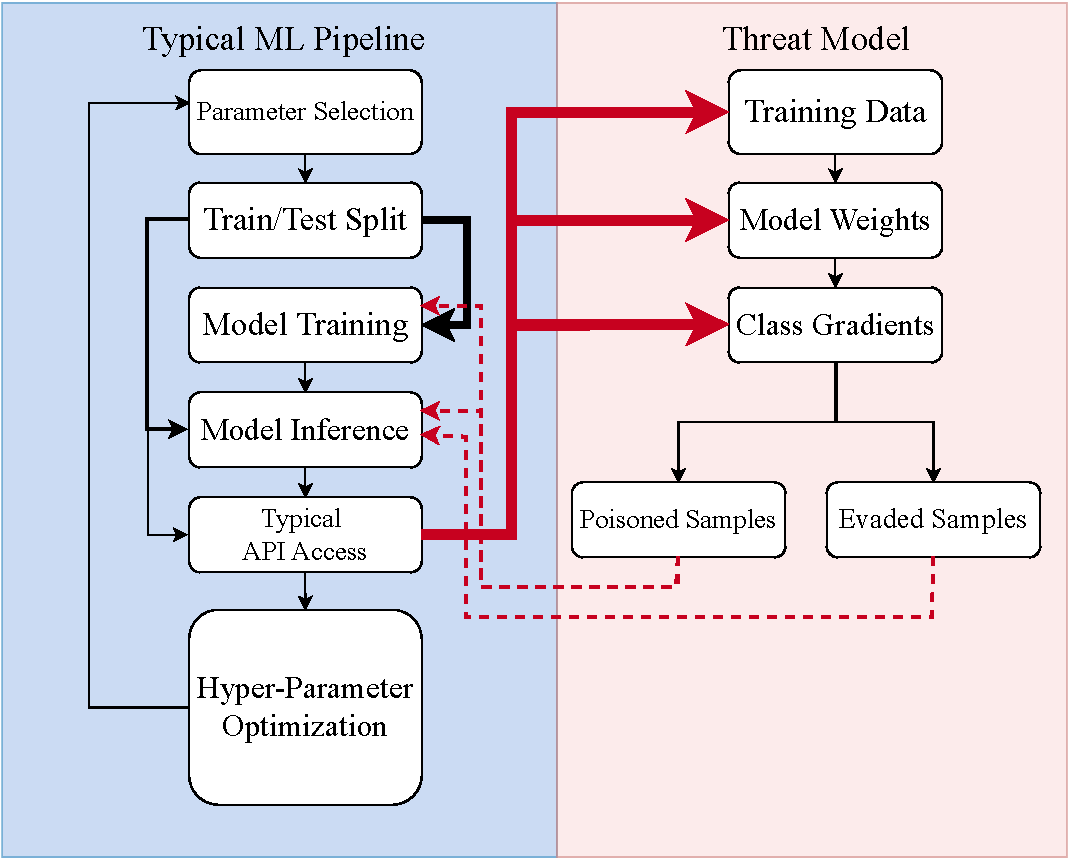
\includegraphics[width=.8\textwidth]{images/attack_diagram.pdf}
    \caption{This diagram depicts the various threat models against a typical machine learning model.}
    \label{fig:threat_model}
\end{figure*}
\label{threat}

% \subsection{Attacks}
% \label{attacks}
% \begin{itemize}
%     \item FGM
%     \item HSJ


% \end{itemize}
% \subsubsection{Attack Related Metrics}
% \paragraph{Minimal Evasion Distance}
% \paragraph{Survival Time}
% % \pargraph{KL_Divergence}
% \paragraph{SHAPr Privacy Metric}
\section{Run-Time Improvements}
\label{improvements}
We can use this model in two different paradigms. In general, the idea is that the number of requisite training samples is very small, so we can run everything client-side, keeping the particulars of the model training private. Another method for distributing the training process, federated learning, trains a model for each user but routinely shares model weights upstream to create a better model for everyone. However, as we outlined in Sec.~\ref{threat}, that opens new attack vectors that would be unsuitable for information the user would like to keep private (\textit{e.g.}, IP address, message contents, or schedule of use). Instead, we propose a few-shot and online methodology for re


\subsection{Real-time, Anomaly Detection}
In some situations, it might be necessary to find anomalies in real-time, which involves special considerations. Namely, we can skip the "training" step entirely and select a number of existing samples from our database for training. These could be selected randomly or according to some time filter in an attempt to only capture new or otherwise unnoticed anomalies. In some cases, it may be that the user doesn't have many samples. However, as we show in the Sec.~\ref{results}, that even small training sets are remarkably effective for this method.



%  Numeric Distances
% \begin{itemize}
%     \item $\ell_0$ (bit-wise distance)
%     \item $\ell_1$ (taxi-driver distance)
%     \item $\ell_2$ (euclidean)
%     \item $\mathscr{\chi}^2$ (weighted difference per entry)
%     \item $\mathscr{L}$ (Laplacian)
%     \item $\mathscr{W}$ (Wasserstein)
% \end{itemize}

\subsubsection{Calculating distance matrix}

While many of the above distance metrics are symmetric, this is not-necessarily the case with NCD. However, if we assume this is true most of the time, we can reduce the computational cost of training and/or prediction. Section~\ref{results} shows how this often improves the accuracy of a model and reduces the number of 



\begin{algorithm}
  \KwData{$X_1$, $X_2$, indexed by $i,j$ respectively.}
  \KwResult{Symmetric distance matrix $S$}
  \BlankLine
  \textbf{Initialize} symmetric matrix $S$ with zeros\;
  \BlankLine
  \ForEach{pair of indices $(i, j) \in \mathcal{D}(X_1, X_2)$ such that $i < j$ }{
    $\mathcal{D}_{ij} \leftarrow \mathcal{D}(X_{1_i}, X_{2_j} )$ \\
    $S_{ij} \leftarrow \matchal{D}_{ij}$ \\
    $S_{ji} \leftarrow \mathcal{D}_{ij}$ \\
  }
  \caption{Compute Symmetric Distance Matrix}
  \label{alg:symmetric-distance-matrix}
\end{algorithm}

% \subsubsection{Removing time-variant noise using autocorellation techniques}

% TODO: talk about arima models


\subsubsection{Pre-computing the Compression vector}
Since the compression step requires the most processing time, we can pre-compute the compression distance for our input data as part of a training step, if we so choose. This offers marginal run-time improvements over the original implementation that repeatedly calculated the NCD of all training samples for each example in the test set. 
See Fig.~\ref{fig:symmetry_time} to see the (signficant) decrease and run-time  and the resulting (marginal) change in accuracy when we pre-compress all of the train and test strings in the data. %Note: this is still running. 










\subsubsection{Reducing the Search Space}
\label{best-samples}
In other situations, it is necessary to minimize the number of samples used for evaluation because the size of the user's database is too large to evaluated in a reasonable amount of time. We can use a variety of heuristics to reduce the size of our search space \cite{amal2011survey}. 
\begin{itemize}
    \item \textbf{Sum:} After calculating the distance matrix, we sort the distance matrix by the sum of a row and find the $m$ most central samples per class.
    \item \textbf{Medoid: }
    \item \textbf{Random : } After calculating the distance matrix, we select $m$ random indices per class.
    \item \textbf{KNN: } After calculating the distance matrix, we use the KNN algorithm to find the $m$-closest neighbors for each class in the training data.
    \item \textbf{SVC: } After calculating the distance matrix, we use a support vector classifier (SVC) to find the indices that define the support-vectors (e.g. the samples that define the class boundaries), then we sort by distance as in \textit{Sum} to find the $m$-most central support vectors to use during the prediction step.
\end{itemize}


\begin{algorithm}
  \caption{Find M-Best Indices}
  \SetAlgoNlRelativeSize{0}
  \SetAlgoNlRelativeSize{-1}
  \SetAlgoNlRelativeSize{-2}
  
  \KwData{Sample points $P$, Number of best indices $m$}
  \KwResult{Set of indices $I$ with the m-best points}
  
  \ForEach{point $p$ in $P$}{
    Calculate a relevance score $r_p$ based on some criterion\;
  }
  
  Sort indices based on relevance scores in descending order: $I \gets$ sortIndices($r_p$)\;
  
  \Return top $m$ indices $I$\;
\end{algorithm}



\subsubsection{Iterative Methods}
We can now treat this as an iterative problem and do a continuous hyperparameter search.



\begin{algorithm}
  \caption{Model Training}
  
  \KwData{System state $S$, Number of iterations $N$, Number of best indices $m$, $x_{test}, y_{test}, X_{train}, y_{train}$}
  \KwResult{Final system state $S$}
  
  Initialize system: $S \gets$ baseline state\;
  \For{$i=1$ to $N$}{
    Sample points: $P \gets$ samplePoints($S$)\;
    Find m-best indices: $I \gets$ findMBestIndices($P, m$)\;
  }
  \Return $m$-best indices, $I$\;
\end{algorithm}







\section{Methods}

\subsection{Datasets}
We examine several to show that this method works well for a variety of anomaly-detection tasks.
\begin{itemize}
    \item KDD-NSL (Intrusion Detection)
    \item Truthseeker (Twitter Bot)
    \item SMS Spam
    \item PCAP DDOS
\end{itemize}
\subsection{Models}

\paragraph{$k$-clusters}
To use KNN, one must specify a number of nearest neighbors to use for class prediction (see: Algorithm~\ref{alg:knn}). We tested $k \in \{1,3,5,7,11\}$, choosing small, odd numbers to make ties impossible for binary classifiers.
\paragraph{Compressors:} In addition to \texttt{gzip}, we tried numerous different compression algorithms. 
\begin{itemize}
    \item gzip - widely available, fast compared to lzma/bz2
    \item lzma - more compression, more time
    \item bz2 - balances gzip/lzma
    \item zstd - designed around real-time usage at the expense of compression depth
\end{itemize}

\paragraph{Training Sample Optimization:}
\label{methods}
We provide theoretical justifications for using secondary methods for determining ideal training set in Section~\ref{improvements}. For the sake of completeness, we tested the mean, medoid, random, KNN, and SVC methods outlined above as well as selecting the $m$-most important samples for each with $m \in$ [10,20,50,100,200,500,1000]. The methods are outlined in full in Sec.~\ref{best-samples}.


\section{Results}

\subsection{Truthseeker}

\subsubsection{Accuracy}
Figure~\ref{fig:accuracy} shows the accuracy of different compressors, metics, and sample selection methods.

\begin{figure*}
	\begin{subfigure}
		\centering
		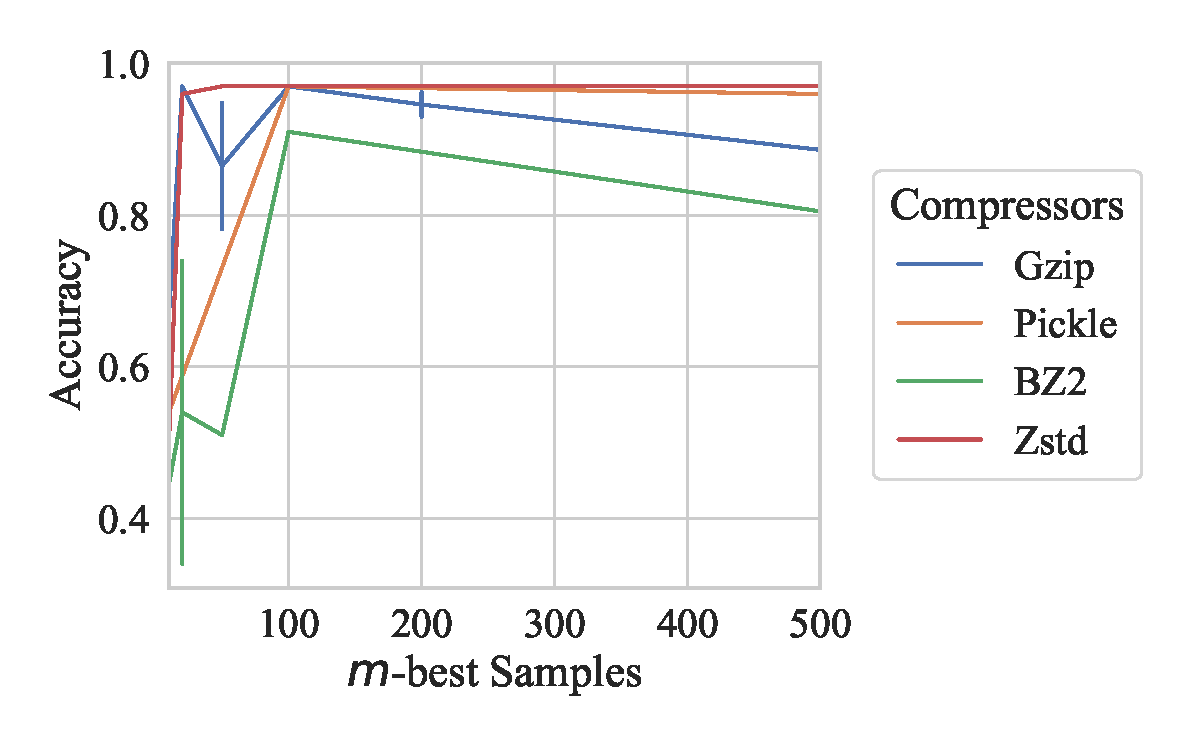
\includegraphics[width=.32\textwidth]{figs/truthseeker/compressor_vs_accuracy.pdf}
	\end{subfigure}%
	~
	\begin{subfigure}
		\centering
		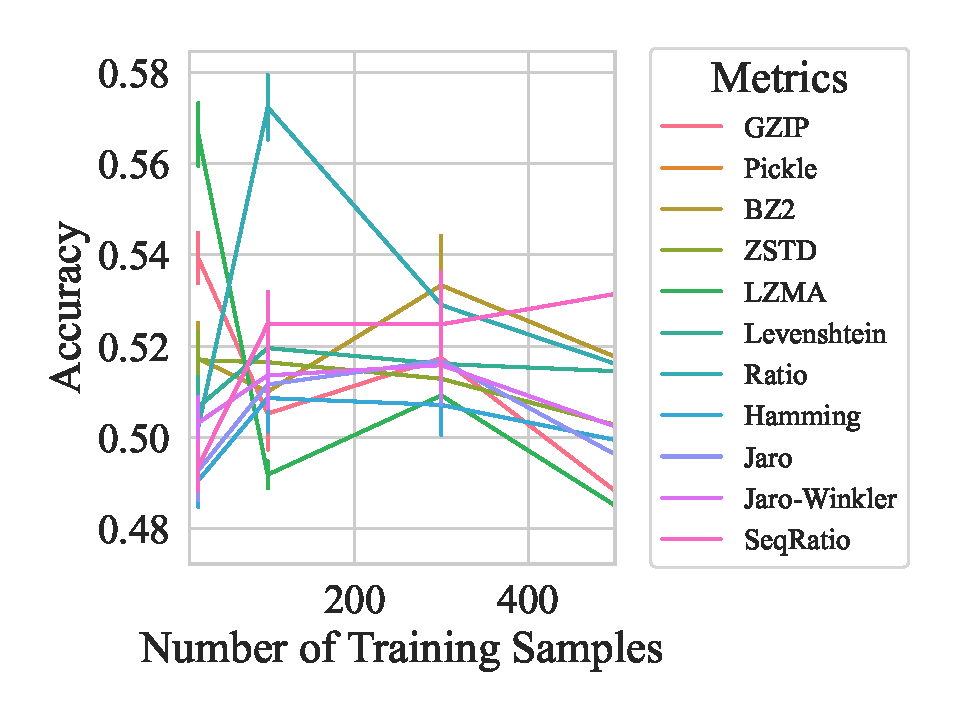
\includegraphics[width=.32\textwidth]{figs/truthseeker/metric_vs_accuracy.pdf}
	\end{subfigure}
	~
	\begin{subfigure}
		\centering
		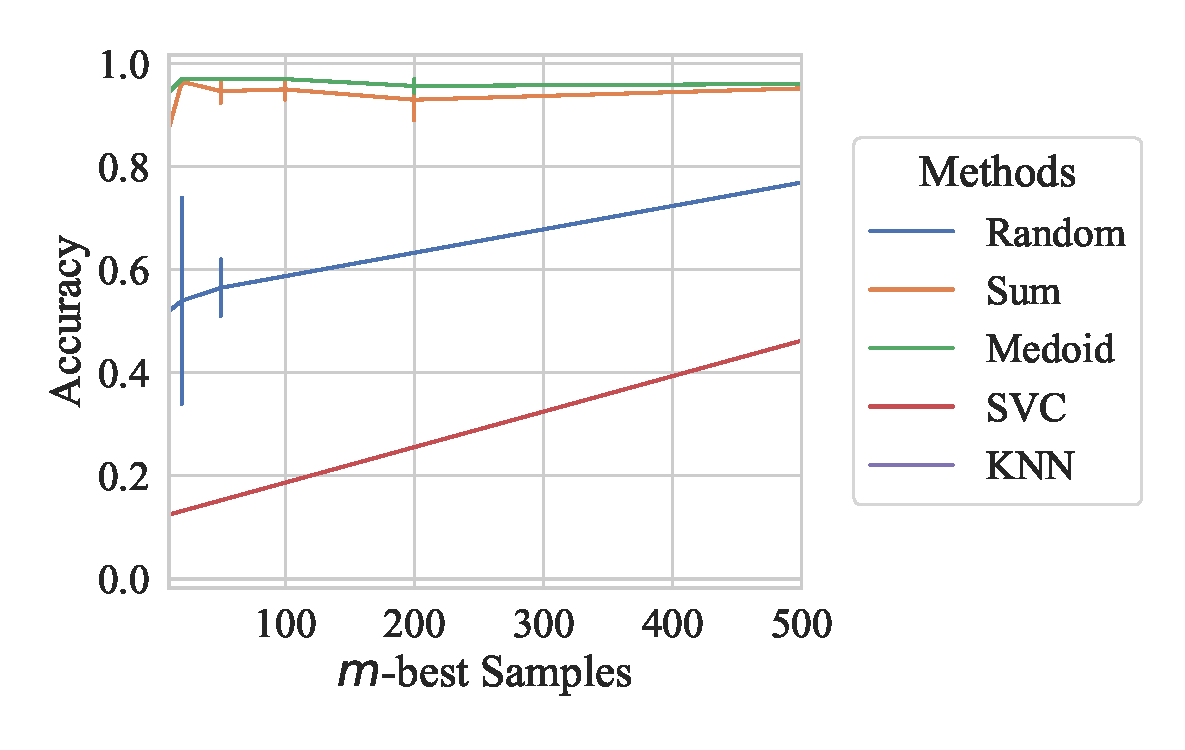
\includegraphics[width=.32\textwidth]{figs/truthseeker/method_vs_accuracy.pdf}
	\end{subfigure}
	\caption{Accuracy across different different compression algorithms (left), distance metrics (center), and sampling methods (right).}
	\label{fig:accuracy}
\end{figure*}

\subsubsection{Training Time}

Figure~\ref{fig:training_time} depicts the training time across all the tested compressors, distance metrics, and sample selection methods.

\begin{figure*}
	\begin{subfigure}
		\centering
		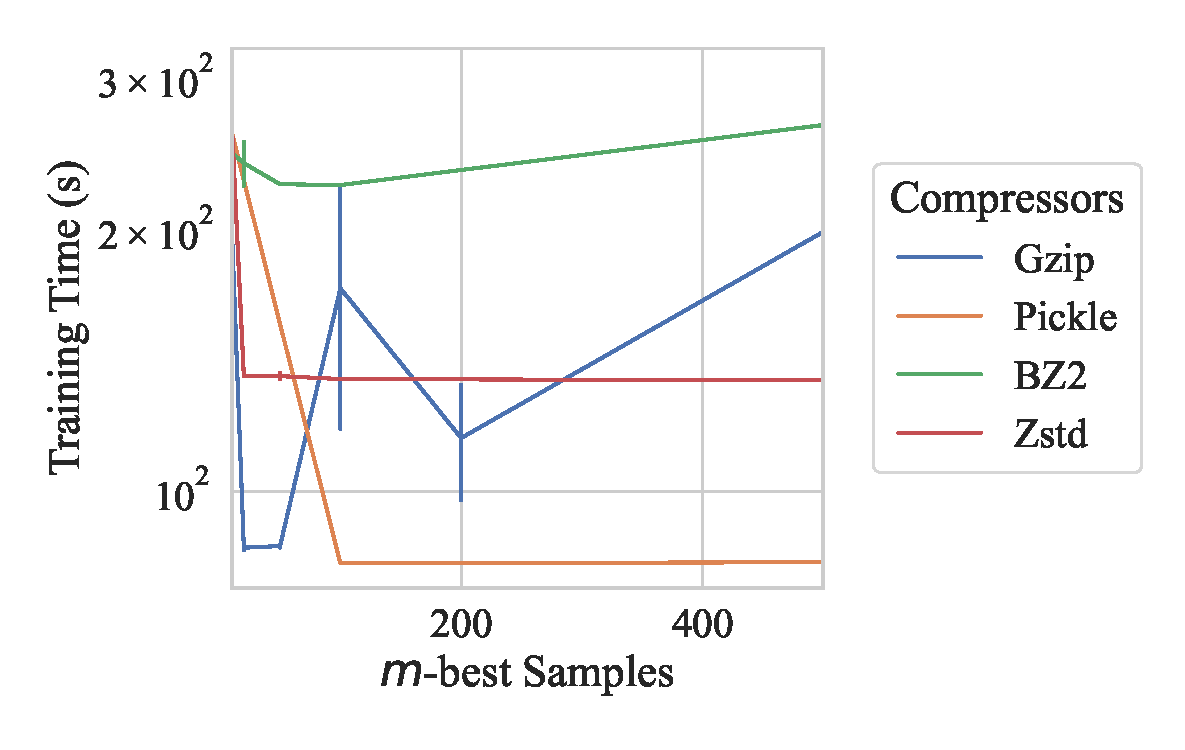
\includegraphics[width=.32\textwidth]{figs/truthseeker/compressor_vs_train_time.pdf}
	\end{subfigure}%
	~
	\begin{subfigure}
		\centering
		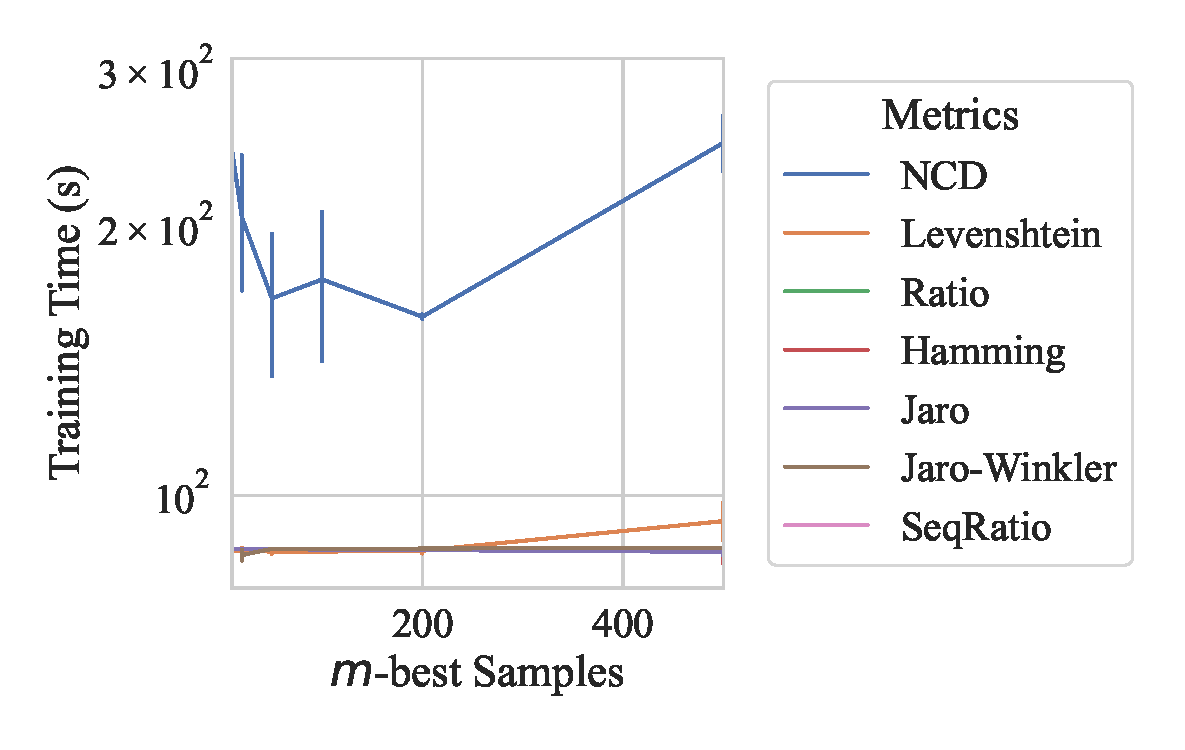
\includegraphics[width=.32\textwidth]{figs/truthseeker/metric_vs_train_time.pdf}
	\end{subfigure}
	~
	\begin{subfigure}
		\centering
		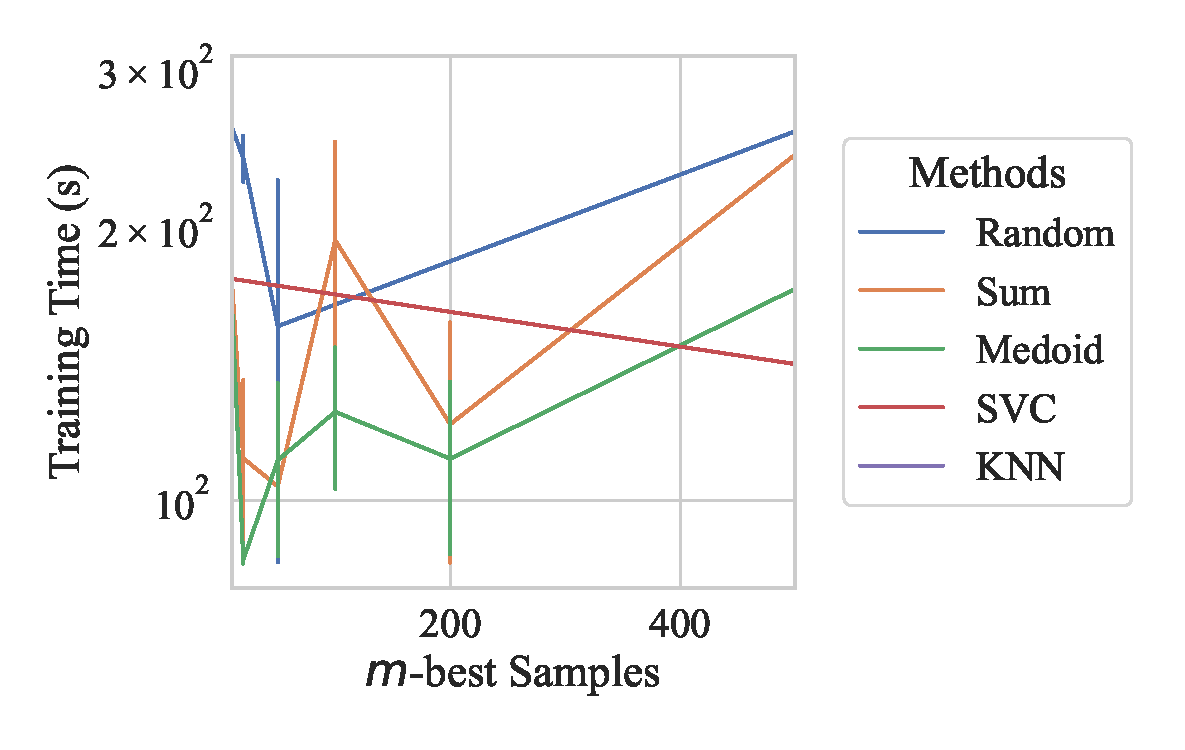
\includegraphics[width=.32\textwidth]{figs/truthseeker/method_vs_train_time.pdf}
	\end{subfigure}
	\caption{Training time across different different compression algorithms (left), distance metrics (center), and sampling methods (right).}
	\label{fig:training_time}
\end{figure*}

\subsubsection{Prediction Time}

Figure~\ref{fig:prediction_time} shows the prediction time of different compressors, metics, and sample selection methods.
\begin{figure*}
	\begin{subfigure}
		\centering
		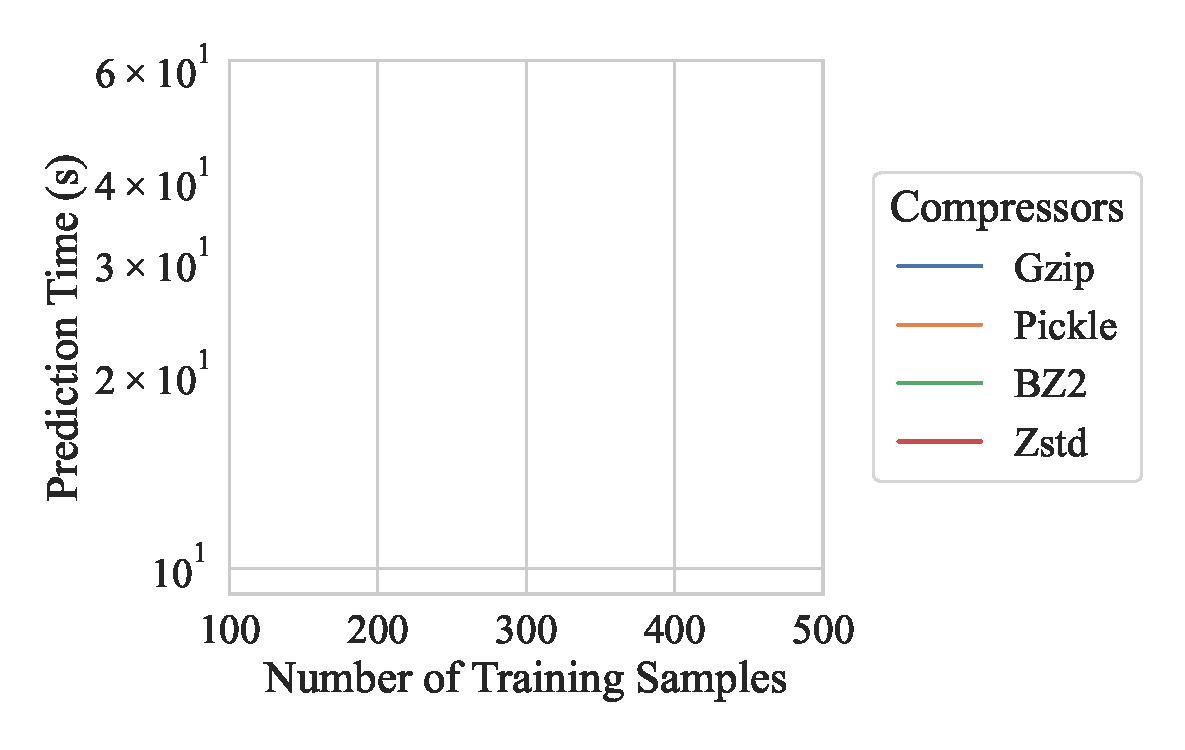
\includegraphics[width=.32\textwidth]{figs/truthseeker/compressor_vs_predict_time.pdf}
	\end{subfigure}%
	~
	\begin{subfigure}
		\centering
		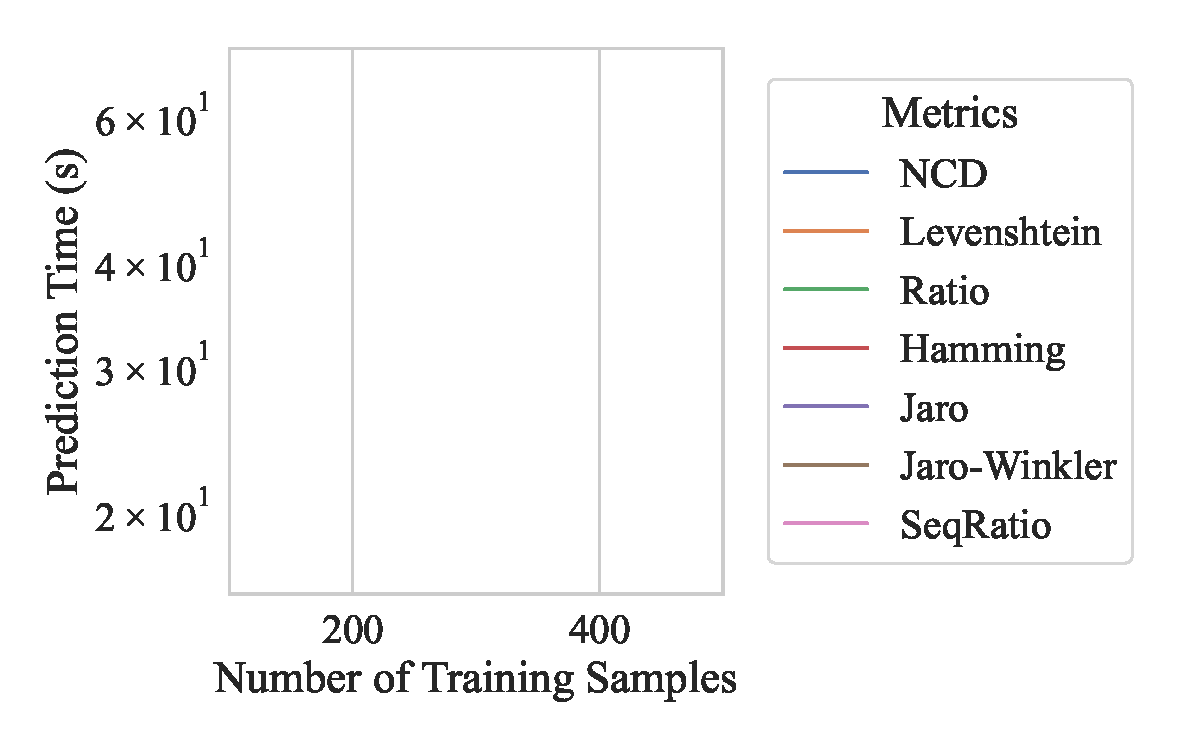
\includegraphics[width=.32\textwidth]{figs/truthseeker/metric_vs_predict_time.pdf}
	\end{subfigure}
	~
	\begin{subfigure}
		\centering
		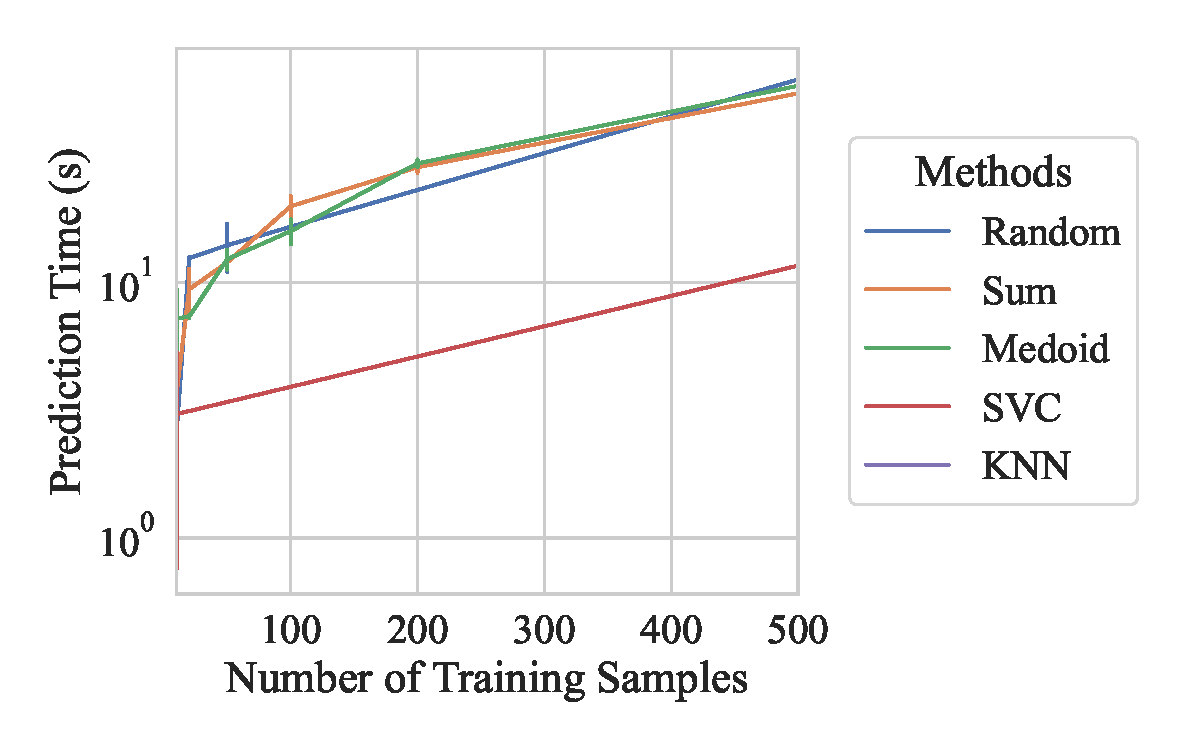
\includegraphics[width=.32\textwidth]{figs/truthseeker/method_vs_predict_time.pdf}
	\end{subfigure}
	\caption{Prediction time across different different compression algorithms (left), distance metrics (center), and sampling methods (right).}.
	\label{fig:prediction_time}
 
\end{figure*}

\subsubsection{Symmetry}

Figure~\ref{fig:symmetry} shows the 

\begin{figure*}
    \begin{subfigure}
        \centering
        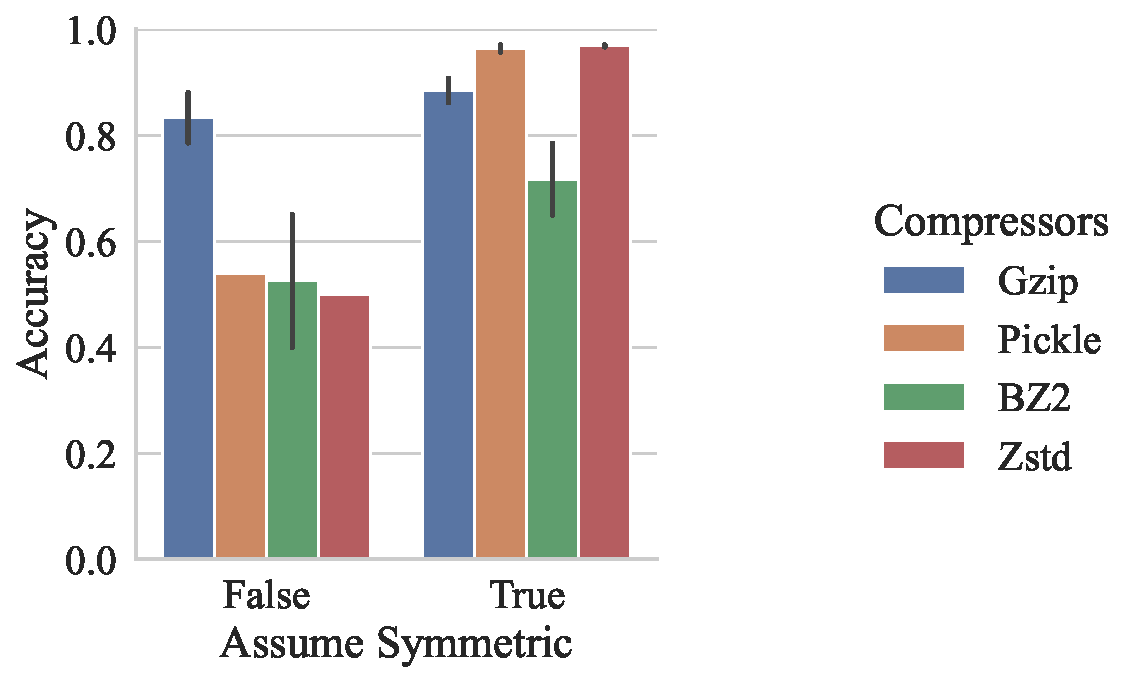
\includegraphics[width=.36\textwidth]{figs/truthseeker/symmetric_vs_compressor.pdf}
    \end{subfigure}
    \begin{subfigure}
        \centering
        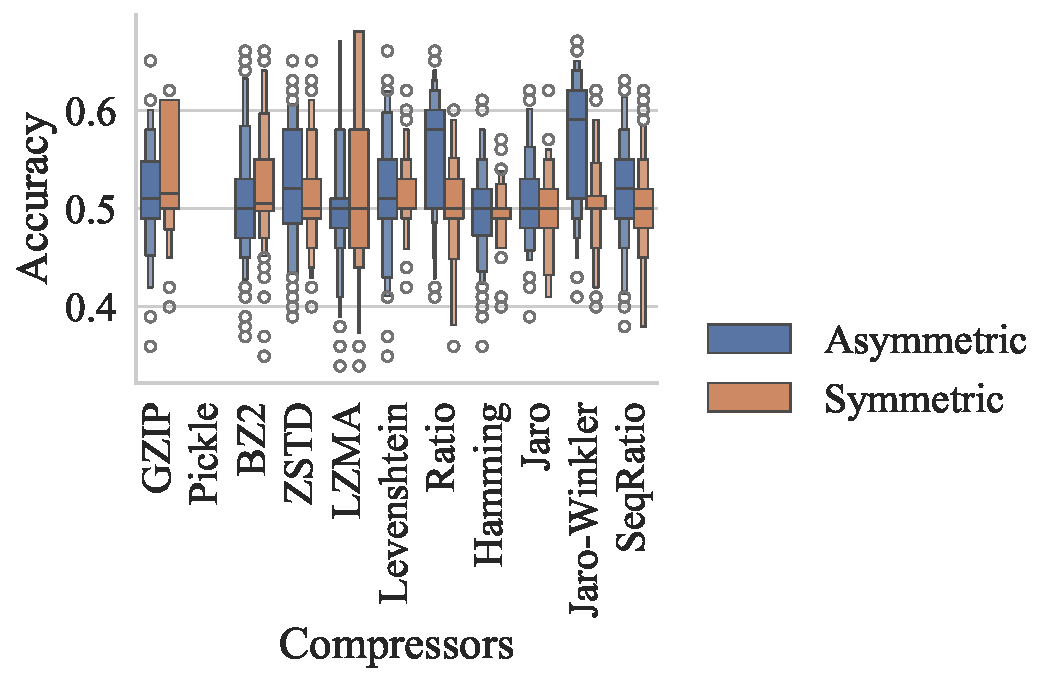
\includegraphics[width=.36\textwidth]{figs/truthseeker/symmetric_vs_metric.pdf}
    \end{subfigure}
    \caption{Accuracy across several compression methods and distance metrics with and without assuming symmetric distances.}
    \label{fig:symmetry}
\end{figure*}

\begin{figure*}
    \begin{subfigure}
        \centering
        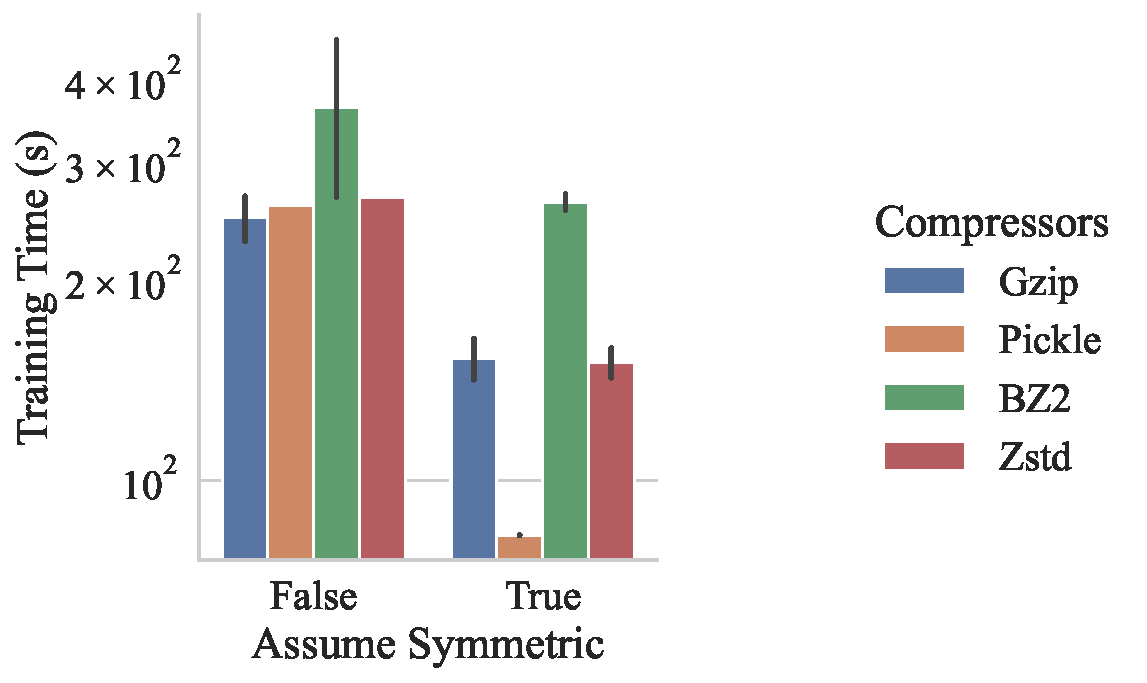
\includegraphics[width=.36\textwidth]{figs/truthseeker/symmetric_vs_compressor_train_time.pdf}
    \end{subfigure}
    \begin{subfigure}
        \centering
        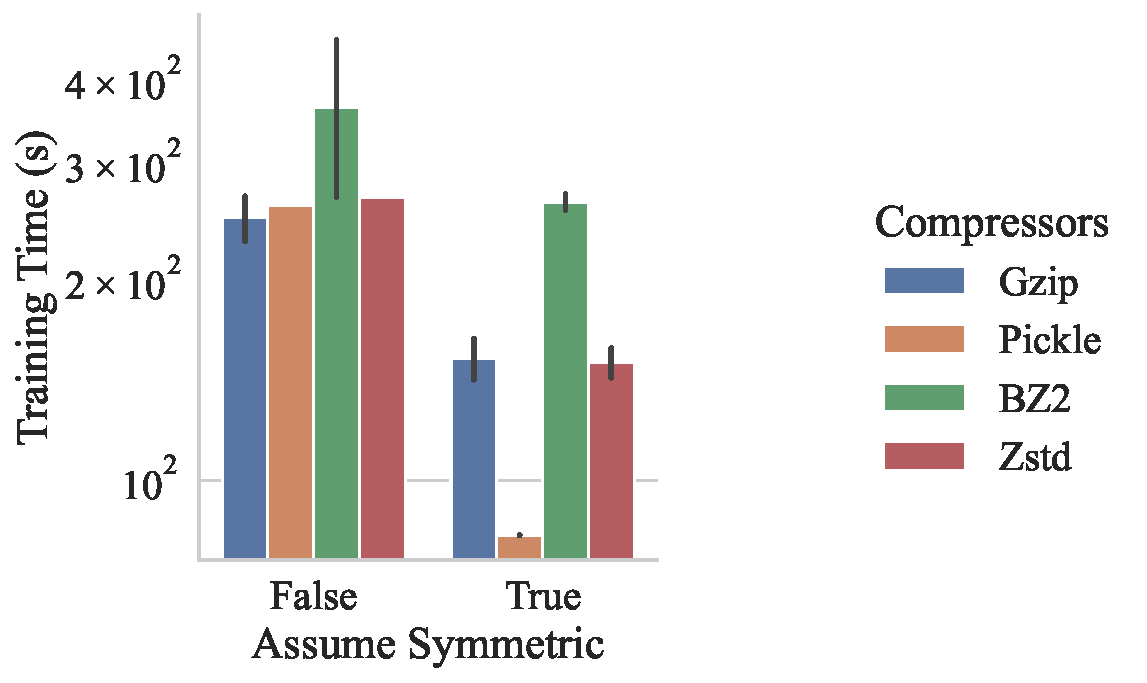
\includegraphics[width=.36\textwidth]{figs/truthseeker/symmetric_vs_compressor_train_time.pdf}
    \end{subfigure}
    \caption{Prediction time across several compression methods and distance metrics with and without assuming symmetric distances.}
    \label{fig:symmetry_time}
\end{figure*}

\subsection{KDD-NSL}

\subsubsection{Accuracy}
Figure~\ref{fig:accuracy} shows the accuracy of different compressors, metics, and sample selection methods.

\begin{figure*}
	\begin{subfigure}
		\centering
		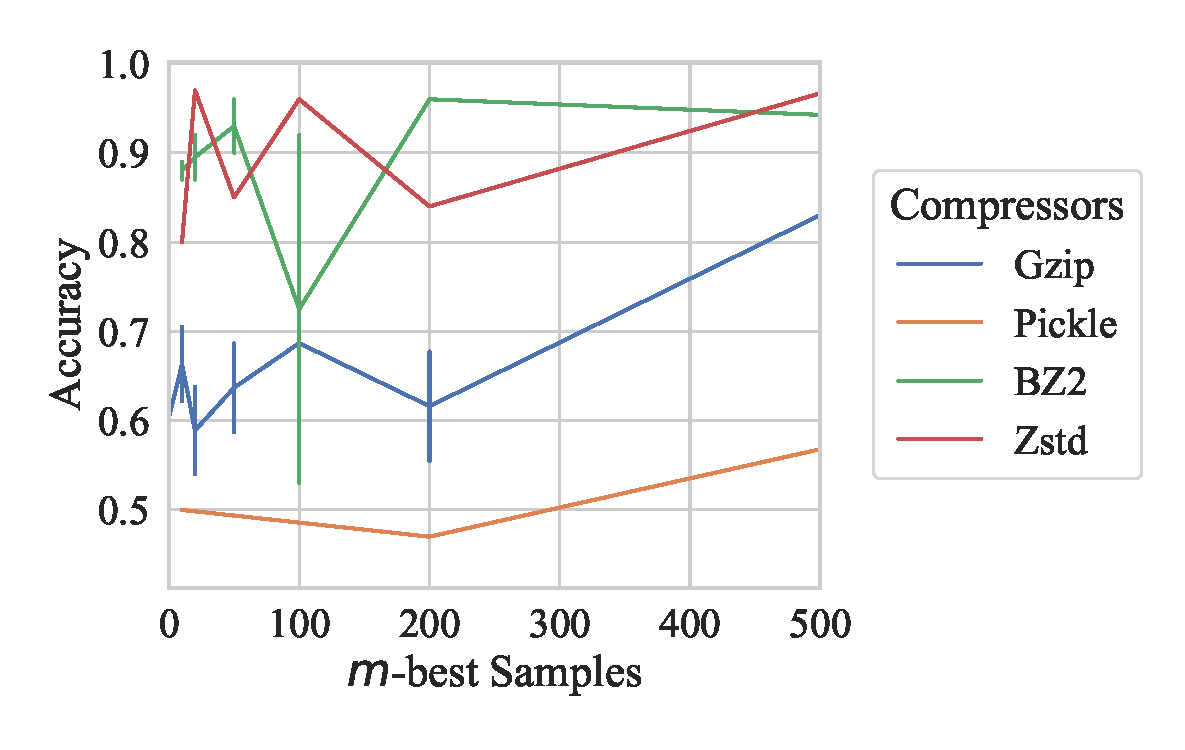
\includegraphics[width=.32\textwidth]{figs/kdd_nsl/compressor_vs_accuracy.pdf}
	\end{subfigure}%
	~
	\begin{subfigure}
		\centering
		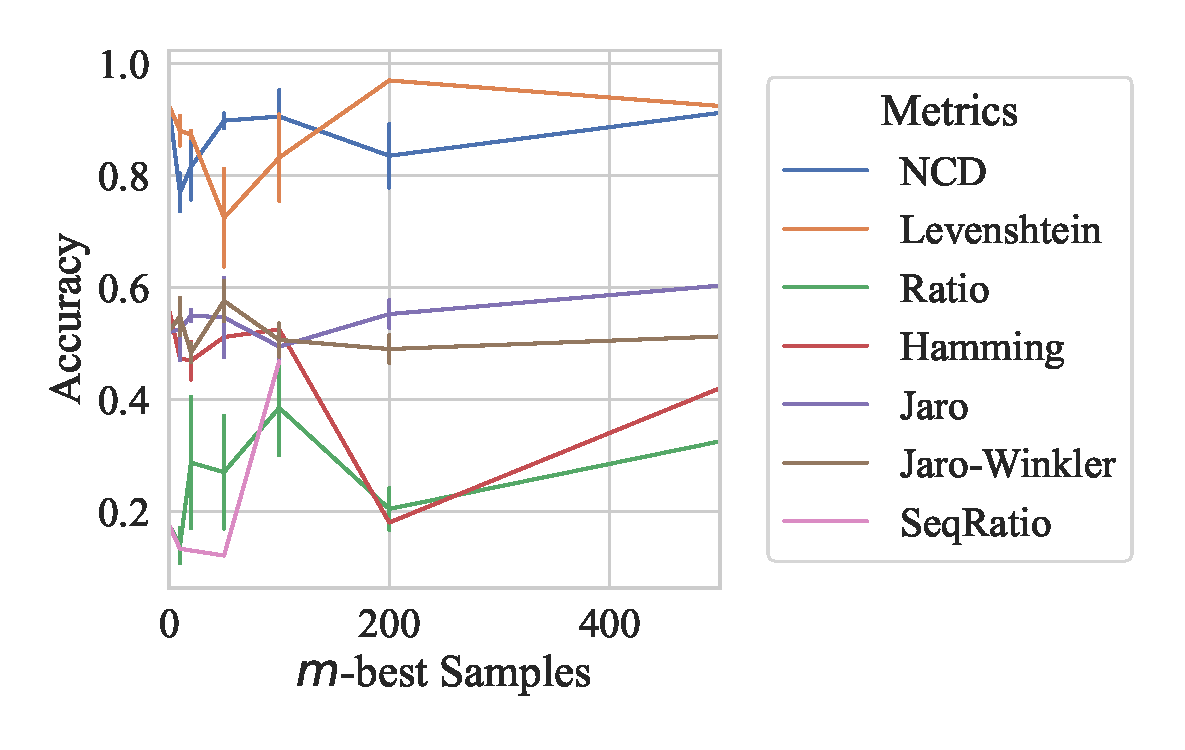
\includegraphics[width=.32\textwidth]{figs/kdd_nsl/metric_vs_accuracy.pdf}
	\end{subfigure}
	~
	\begin{subfigure}
		\centering
		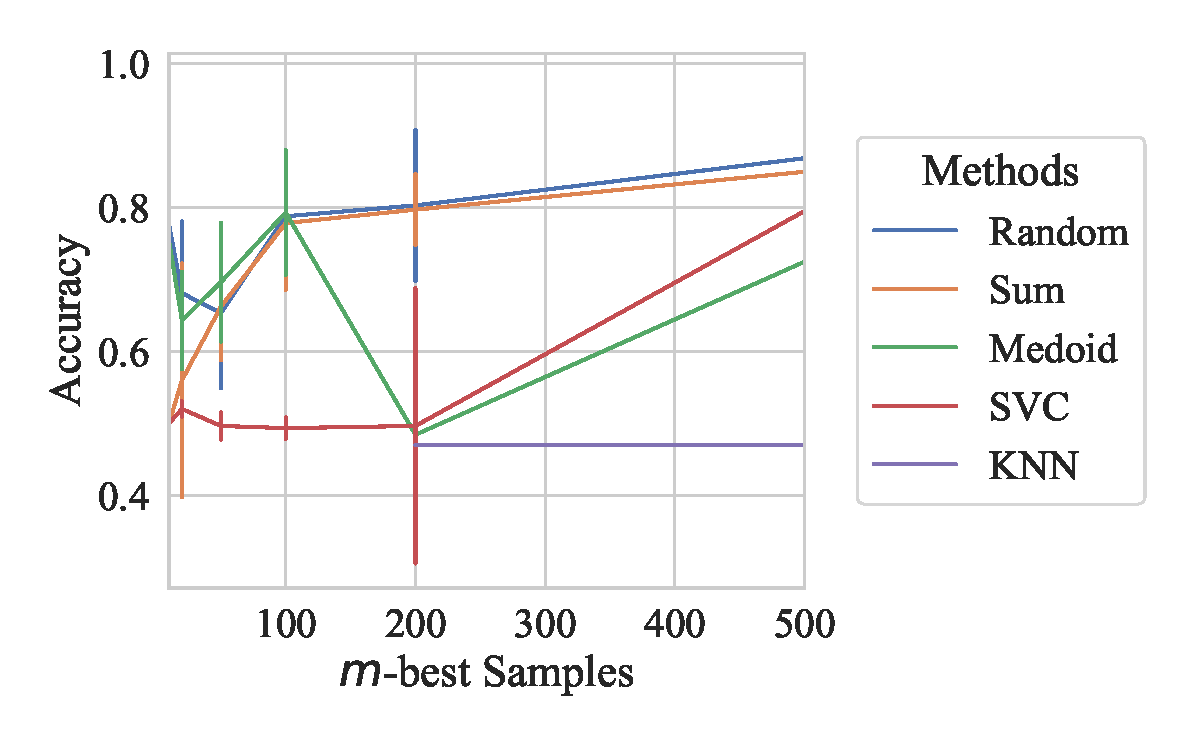
\includegraphics[width=.32\textwidth]{figs/kdd_nsl/method_vs_accuracy.pdf}
	\end{subfigure}
	\caption{Accuracy across different different compression algorithms (left), distance metrics (center), and sampling methods (right).}
	\label{fig:accuracy_kdd}
\end{figure*}

\subsubsection{Training Time}

Figure~\ref{fig:training_time} depicts the training time across all the tested compressors, distance metrics, and sample selection methods.

\begin{figure*}
	\begin{subfigure}
		\centering
		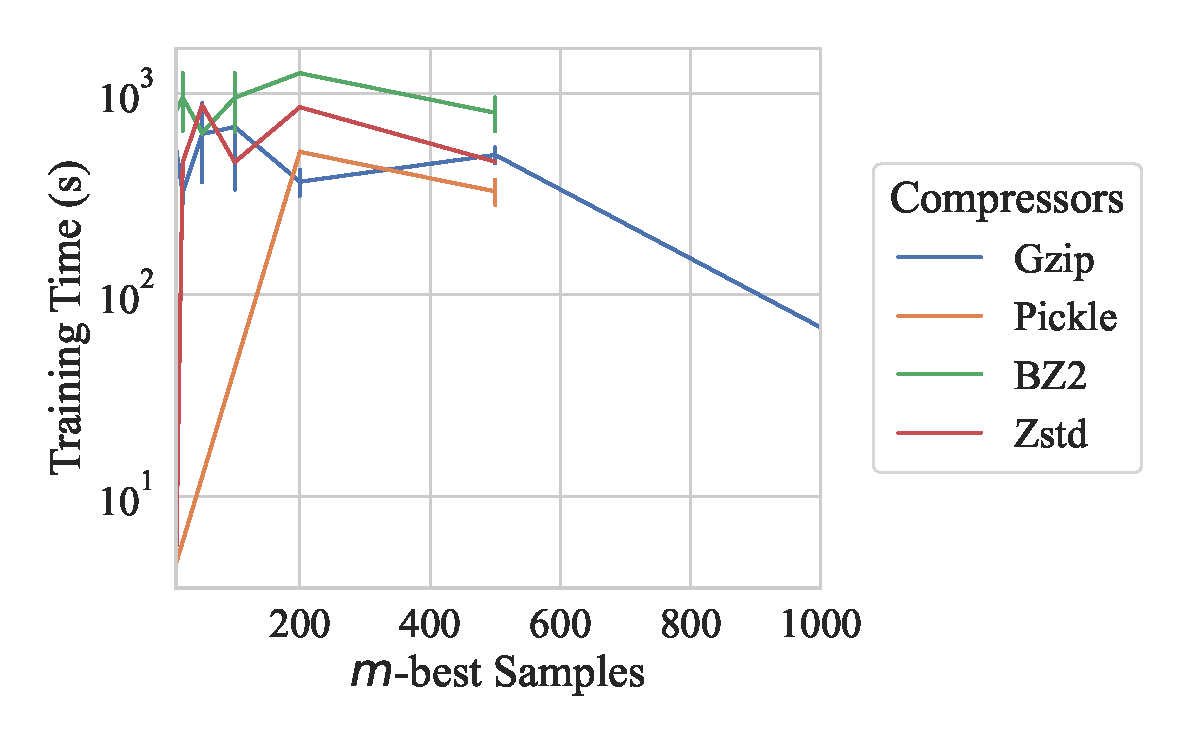
\includegraphics[width=.32\textwidth]{figs/kdd_nsl/compressor_vs_train_time.pdf}
	\end{subfigure}%
	~
	\begin{subfigure}
		\centering
		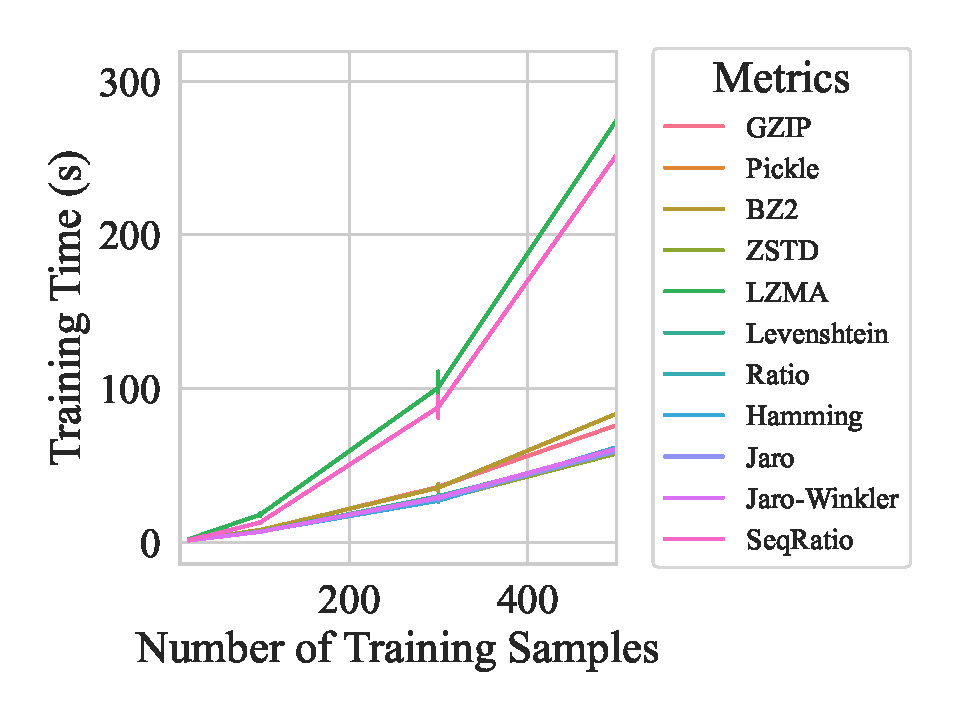
\includegraphics[width=.32\textwidth]{figs/kdd_nsl/metric_vs_train_time.pdf}
	\end{subfigure}
	~
	\begin{subfigure}
		\centering
		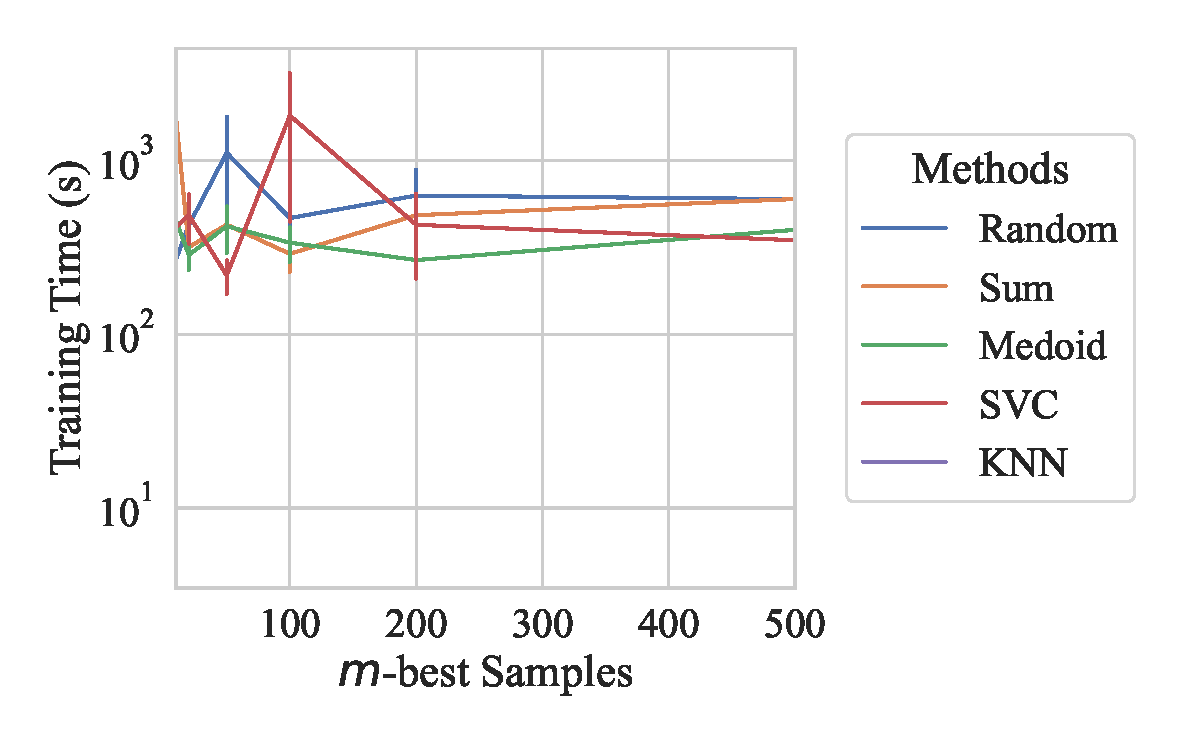
\includegraphics[width=.32\textwidth]{figs/kdd_nsl/method_vs_train_time.pdf}
	\end{subfigure}
	\caption{Training time across different different compression algorithms (left), distance metrics (center), and sampling methods (right).}
	\label{fig:training_time_kdd}
\end{figure*}

\subsubsection{Prediction Time}

Figure~\ref{fig:prediction_time} shows the prediction time of different compressors, metics, and sample selection methods.
\begin{figure*}
	\begin{subfigure}
		\centering
		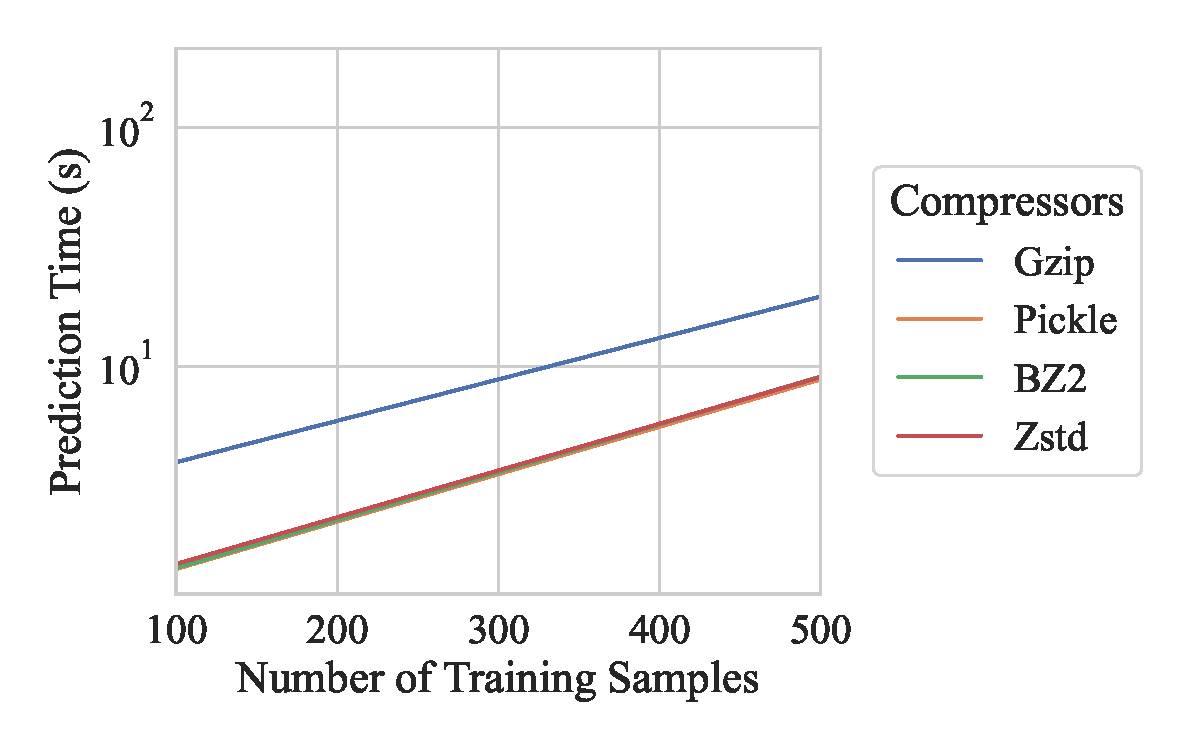
\includegraphics[width=.32\textwidth]{figs/kdd_nsl/compressor_vs_predict_time.pdf}
	\end{subfigure}%
	~
	\begin{subfigure}
		\centering
		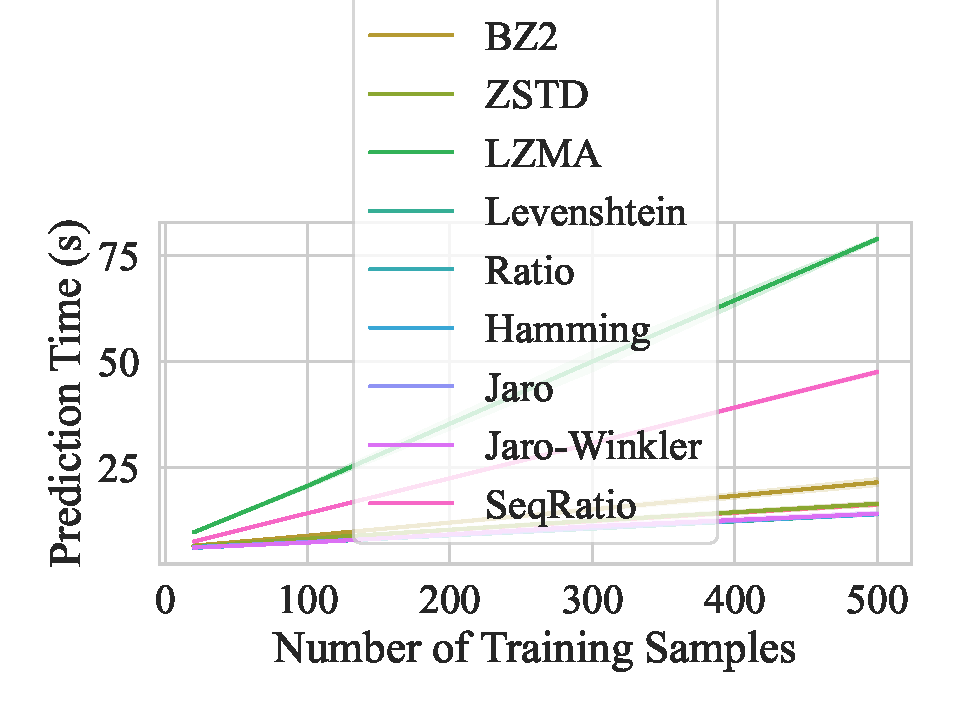
\includegraphics[width=.32\textwidth]{figs/kdd_nsl/metric_vs_predict_time.pdf}
	\end{subfigure}
	~
	\begin{subfigure}
		\centering
		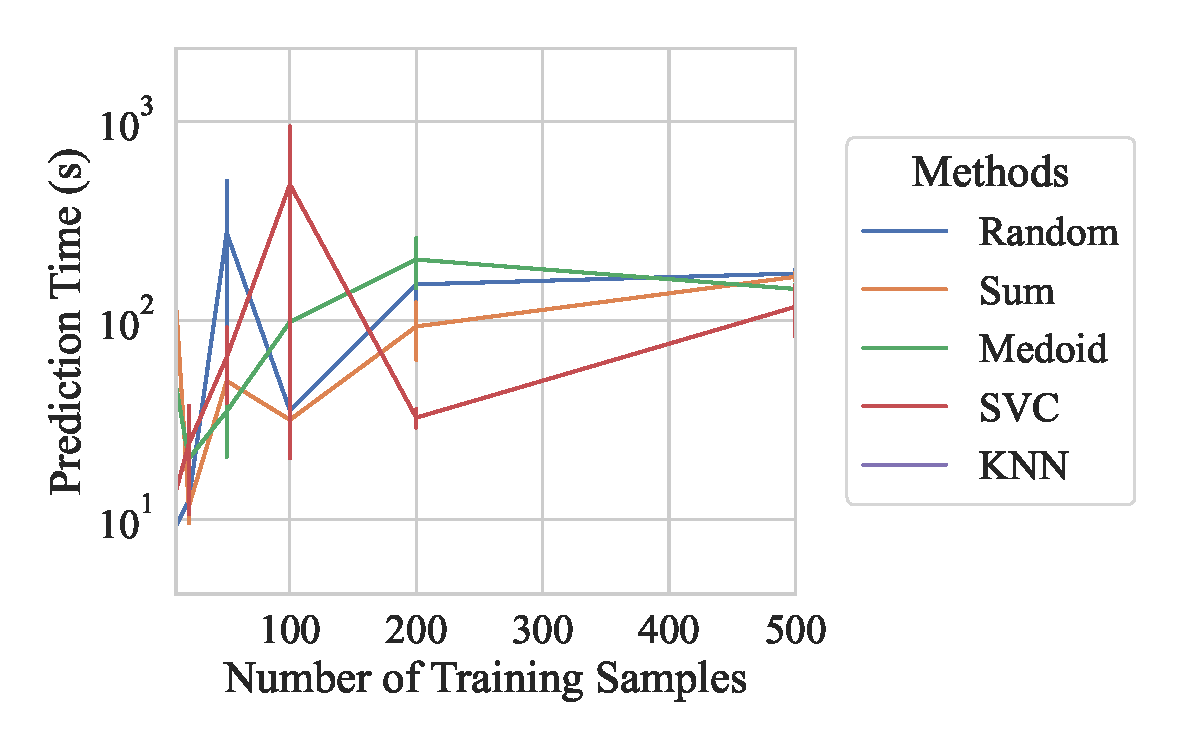
\includegraphics[width=.32\textwidth]{figs/kdd_nsl/method_vs_predict_time.pdf}
	\end{subfigure}
	\caption{Prediction time across different different compression algorithms (left), distance metrics (center), and sampling methods (right).}.
	\label{fig:prediction_time_kdd}
\end{figure*}

\subsubsection{Symmetry}


\begin{figure*}
    \begin{subfigure}
        \centering
        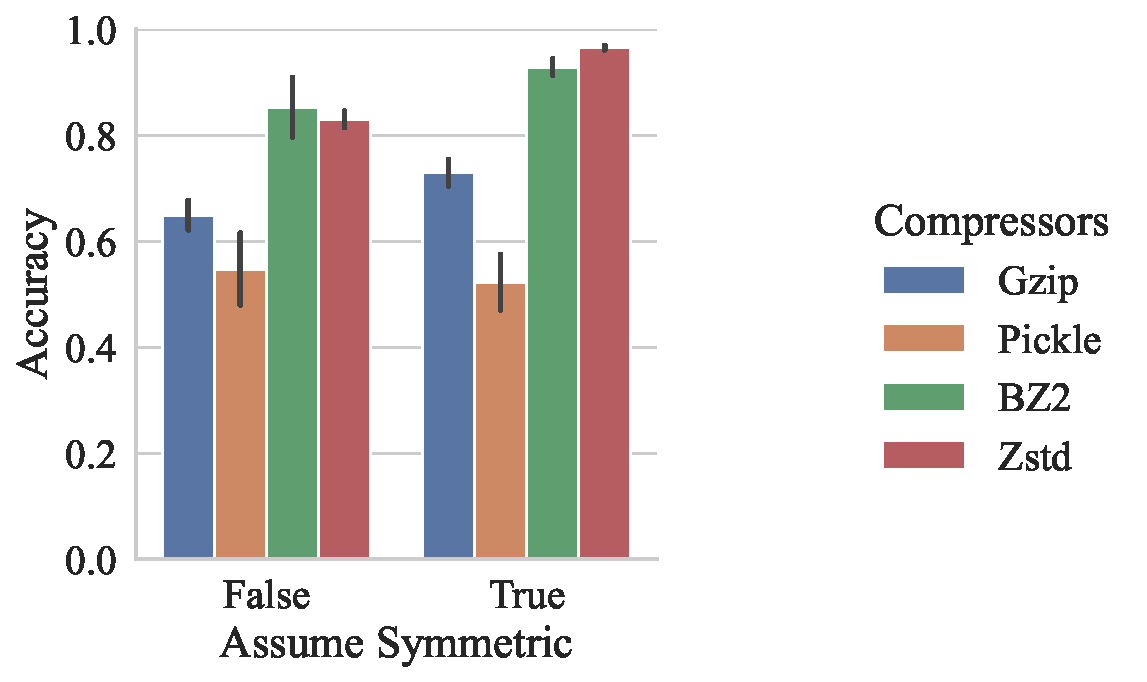
\includegraphics[width=.36\textwidth]{figs/kdd_nsl/symmetric_vs_compressor.pdf}
    \end{subfigure}
    \begin{subfigure}
        \centering
        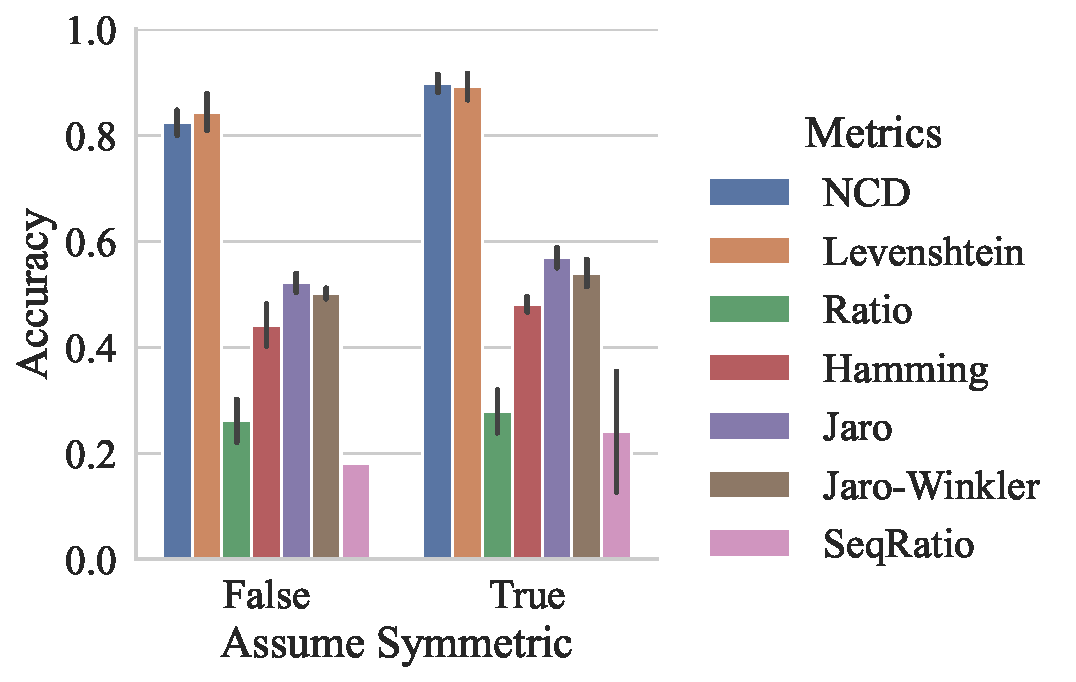
\includegraphics[width=.36\textwidth]{figs/kdd_nsl/symmetric_vs_metric.pdf}
    \end{subfigure}
    \caption{Accuracy across several compression methods and distance metrics with and without assuming symmetric distances.}
    \label{fig:symmetry_kdd}
\end{figure*}

\label{results}
\section{Considerations}
\label{considerations}
\section{Conclusion}
\label{conclusion}


\bibliographystyle{ieeetr}
\clearpage
\bibliography{acmart}

\end{document}
\endinput
%%
